\chapter{Algorytm diagnozowania kręgozmyku i tyłozmyku}

\section{Kliniczna charakterystyka kręgozmyku i tyłozmyku}

Kręgozmyk (łac. \textit{spondylolisthesis}, z gr. \textit{spondylos} -- kręg, \textit{olisthesis} -- ześlizg) definiowany jest jako przemieszczenie trzonu kręgu ku przodowi względem kręgu leżącego poniżej, obserwowane w płaszczyźnie strzałkowej.\cite{gagnet}
Przeciwieństwem tej patologii jest tyłozmyk (ang. \textit{retrolisthesis}), w którym przemieszczenie następuje w kierunku tylnym.
Obydwa stany prowadzą do zaburzenia prawidłowej osi biomechanicznej kręgosłupa, a w zaawansowanych przypadkach -- do zwężenia kanału kręgowego i ucisku struktur nerwowych.

Powszechnie stosowana klasyfikacja Wiltse'a, Newmana i Macnaba\cite{wiltse} wyróżnia pięć typów kręgozmyku ze względu na mechanizm powstawania:

\begin{itemize}
    \item \textbf{dysplastyczny} -- wynikający z wrodzonej wady budowy stawów międzykręgowych lub tylnego łuku kręgu; rozpoznawany zazwyczaj w dzieciństwie,
    \item \textbf{cieśniowy} (istmiczny) -- spowodowany przerwaniem ciągłości części międzystawowej łuku kręgowego (łac. \textit{pars interarticularis}, spondylolizą); najczęstszy typ u osób młodych, szczególnie narażonych na przeciążenia osiowe,
    \item \textbf{zwyrodnieniowy} -- będący konsekwencją degeneracji krążków międzykręgowych oraz stawów międzykręgowych; dominujący typ u osób po 50. roku życia i najczęściej spotykany w zbiorze danych analizowanym w niniejszej pracy,
    \item \textbf{pourazowy} -- następstwo złamania elementów tylnych kręgu innych niż część międzystawowa,
    \item \textbf{patologiczny} -- wynikający z miejscowej lub uogólnionej choroby kości, np. nowotworowej lub metabolicznej.
\end{itemize}

Kręgozmyk zwyrodnieniowy dotyczy przede wszystkim poziomów L4/L5 i L5/S1, gdzie obciążenie mechaniczne kręgosłupa jest największe.
Degeneracja krążka międzykręgowego prowadzi do niestabilności segmentu ruchowego, a wtórne zmiany w stawach międzykręgowych nie są w stanie skutecznie ograniczyć patologicznego ruchu trzonów\cite{akkawi}.
Tyłozmyk zwyrodnieniowy występuje rzadziej niż kręgozmyk przedni i częściej towarzyszy mu wielopoziomowe zwężenie kanału kręgowego.

Objawy kliniczne zależą od stopnia przemieszczenia i poziomu zajętego odcinka.
Najczęstszą dolegliwością jest ból w dolnej części pleców, nasilający się podczas stania i chodzenia, a ustępujący w pozycji siedzącej lub przy nachyleniu tułowia do przodu.
Przy ucisku korzeni nerwowych dołącza się ból promieniujący do kończyn dolnych (rwa kulszowa lub udowa), zaburzenia czucia oraz osłabienie siły mięśniowej.

Diagnostyka obrazowa kręgozmyku opiera się przede wszystkim na zdjęciu rentgenowskim kręgosłupa lędźwiowo-krzyżowego wykonanym w projekcji bocznej w pozycji stojącej.
Takie badanie uwzględnia obciążenie grawitacyjne kręgosłupa, które może nasilać przemieszczenie w porównaniu z badaniem w pozycji leżącej.
Rezonans magnetyczny stanowi uzupełnienie diagnostyki, umożliwiając ocenę stopnia ucisku worka oponowego, korzeni nerwowych oraz stanu krążków międzykręgowych.
To właśnie dane z badań MRI, po przeprowadzonej segmentacji, stanowią wejście dla algorytmu opisanego w niniejszym rozdziale.

Ilościową ocenę stopnia przemieszczenia kręgu przeprowadza się metodą Meyerdinga\cite{koslosky}, która dzieli kręgozmyk na cztery stopnie w zależności od odsetka przesunięcia trzonu kręgu w stosunku do szerokości górnej powierzchni kręgu leżącego poniżej.
W tym celu na bocznym zdjęciu RTG wyznacza się tylny obrys trzonu kręgu górnego i dolnego, a wartość ześlizgu wyraża się jako iloraz odległości między tylnymi krawędziami trzonów do szerokości górnej płytki granicznej kręgu dolnego.
Stopniowanie przedstawiono w tabeli~\ref{tab:meyerding}.

\begin{table}[H]
\centering
\caption{Klasyfikacja kręgozmyku według skali Meydinga}
\label{tab:meyerding}
\begin{tabular}{ccc}
\hline
\textbf{Stopień} & \textbf{Przemieszczenie} & \textbf{Opis kliniczny} \\
\hline
I   & 0--25\%   & łagodny, często bezobjawowy \\
II  & 25--50\%  & umiarkowany, zazwyczaj objawowy \\
III & 50--75\%  & znaczny, zwężenie kanału kręgowego \\
IV  & 75--100\% & ciężki, wyraźne objawy neurologiczne \\
\hline
\end{tabular}
\end{table}

W niektórych ujęciach skalę uzupełnia się o stopień V (spondyloptoza), odpowiadający całkowitemu zsunięciu trzonu kręgu poniżej powierzchni kręgu leżącego niżej (przemieszczenie powyżej 100\%).\cite{koslosky}

Pomiar według Meyerdinga jest prosty i powtarzalny, jednak obarczony pewną zmiennością obserwatora wynikającą z trudności w precyzyjnym wyznaczeniu obrysów trzonów na dwuwymiarowym zdjęciu RTG.\cite{tallroth}
Ponadto standardowa projekcja boczna nie uwzględnia rotacji osiowej kręgów, która może towarzyszyć kręgozmykowi zwłaszcza w przebiegu skoliozy.

Algorytm opisany w niniejszym rozdziale realizuje automatyczny pomiar analogiczny do metody Meyerdinga, operując jednak na trójwymiarowej segmentacji MRI zamiast dwuwymiarowego zdjęcia RTG.
Wyznaczone punkty narożne trzonów kręgów pozwalają na obliczenie znormalizowanego przesunięcia w płaszczyźnie strzałkowej każdego kręgu, bez konieczności ręcznego wskazywania struktur anatomicznych przez radiologa.

Należy przy tym pamiętać, że badanie MRI wykonywane jest w pozycji leżącej, w której obciążenie grawitacyjne kręgosłupa jest mniejsze niż podczas stojącego zdjęcia RTG; wartość ześlizgu wyznaczona na podstawie segmentacji MRI może być więc niedoszacowana względem pomiaru w warunkach obciążenia.

\section{Założenia funkcjonalne i niefunkcjonalne}

Algorytm detekcji kręgozmyku i tyłozmyku współdzieli szereg założeń z algorytmem detekcji skoliozy opisanym w rozdziale~\ref{chap:skolioza}.
Dotyczy to w szczególności: obsługi wolumetrycznych danych wejściowych w formacie NIfTI, wyznaczania linii środkowej kanału kręgowego, ekstrakcji przekrojów 2D wraz z detekcją punktów narożnych trzonu, eksportu wyników w formacie JSON kompatybilnym z~oprogramowaniem 3D~Slicer, a~także wymagań dotyczących odporności na nieciągłości w segmentacji, powtarzalności wyników oraz efektywności czasowej przetwarzania.

Wymagania funkcjonalne:

\begin{itemize}
    \item \textbf{Rekonstrukcja linii środkowej o równomiernym próbkowaniu} -- krzywa kanału kręgowego jest poddawana uzupełnieniu luk i reparametryzowana według kumulatywnej długości łuku, co zapewnia równomierne rozmieszczenie punktów referencyjnych wzdłuż kanału.
    \item \textbf{Pomiar znormalizowanego przesunięcia strzałkowego} -- algorytm oblicza przemieszczenie górnego trzonu kręgu względem dolnego.
    Wynik jest wartością bezwymiarową z przedziału $[0, 1]$, interpretowaną jako odsetek szerokości trzonu kręgu dolnego -- analogicznie do skali Meyerdinga stosowanej w pomiarach na zdjęciach RTG.
    \item \textbf{Klasyfikacja kierunku przesunięcia} -- na podstawie znaku rzutu algorytm rozróżnia kręgozmyk (przemieszczenie do przodu, \textit{spondylolisthesis}) od tyłozmyku (przemieszczenie do tyłu, \textit{retrolisthesis}).
    \item \textbf{Analiza wszystkich par sąsiednich kręgów} -- pomiar wykonywany jest dla każdej pary kolejnych kręgów obecnych w segmentacji (Th11--S1); wynik zwracany jest osobno dla każdego poziomu.
\end{itemize}

Wymagania niefunkcjonalne:
\begin{itemize}
    \item \textbf{Odporność na nieciągłości segmentacji kanału kręgowego} -- algorytm wypełnia luki w szkielecie kanału kręgowego wynikające ze słabej jakości segmentacji lub obecności artefaktów w badaniu MRI.
    \item \textbf{Niezależność od orientacji przestrzennej kręgosłupa} -- algorytm oblicza poprawny wynik niezależnie od globalnego pochylenia i rotacji kręgosłupa w przestrzeni skanera, a tym samym niezależnie od ułożenia pacjenta podczas badania.
    \item \textbf{Niezależność wyniku od skali przestrzeni obrazowej} -- algorytm zwraca poprawne wyniki niezależnie od parametrów aparatu MRI takich jak rozdzielczość wokseli.
    \item \textbf{Powtarzalność wyników} -- dla tych samych danych wejściowych algorytm musi zwracać zawsze ten sam wynik pomiarowy, bez elementów losowych.
    \item \textbf{Pełna automatyzacja} -- proces pomiaru musi przebiegać bez interakcji manualnej, w szczególności bez ręcznego wskazywania kręgów ani wyznaczania obrysów trzonów przez użytkownika.
    \item \textbf{Efektywność czasowa przetwarzania} -- czas przetwarzania pojedynczego badania nie powinien przekraczać wartości akceptowalnej w kontekście wspomagania diagnostyki klinicznej.
\end{itemize}

Realizację powyższych wymagań opisano w kolejnych podrozdziałach, przedstawiając kolejne etapy przetwarzania danych od wczytania segmentacji do wyznaczenia wartości przesunięcia.

\section{Metodyka i opis algorytmu}
\label{sec:kregozmyk-metodyka}

Algorytm pomiaru przesunięcia w płaszczyźnie strzałkowej korzysta z tego samego potoku przetwarzania danych, który przedstawiono w rozdziale~\ref{chap:skolioza}.
Wspólne pozostają trzy pierwsze etapy: rekonstrukcja linii środkowej kanału kręgowego, wyznaczenie lokalnego układu współrzędnych kręgu oraz ekstrakcja przekroju dwuwymiarowego wraz z detekcją punktów narożnych trzonu.
Różnice dotyczą doboru płaszczyzny pomiarowej, sposobu zestawiania kręgów w pary oraz samego pomiaru, którego wynikiem nie jest kąt, lecz bezwymiarowa wielkość opisująca względne przemieszczenie trzonów.
W niniejszym podrozdziale etapy wspólne omówiono skrótowo, wraz z zestawieniem różnic w parametrach, natomiast szczegółowo opisano wyłącznie części specyficzne dla detekcji kręgozmyku i tyłozmyku.

\begin{figure}[H]
    \centering
    % TODO: podmienić na obrazy/spondylolisthesis_pipeline.jpg
    \fbox{\parbox[c][5cm][c]{0.9\textwidth}{\centering\textit{miejsce na schemat potoku przetwarzania}}}
    \captionsetup{justification=centering, font=small}
    \caption{Ogólny potok przetwarzania danych dla algorytmu detekcji kręgozmyku i tyłozmyku}
    \label{fig:spondylolisthesis-pipeline}
\end{figure}

\subsection{Etapy wspólne z algorytmem detekcji skoliozy}
\label{subsec:wspolne-etapy}

Pierwszym etapem jest wyznaczenie linii środkowej kanału kręgowego, opisane w podrozdziale~\ref{subsec:centerline}.
Trzy etykiety segmentacji składające się na kanał kręgowy scalane są w jedną strukturę, która następnie poddawana jest szkieletyzacji metodą Lee.
Centroidy kolejnych warstw poprzecznych szkieletu tworzą uporządkowany zbiór punktów, w którym luki wynikające z niedoskonałości segmentacji uzupełniane są interpolacją funkcjami sklejanymi trzeciego stopnia, a całość podlega reparametryzacji według skumulowanej długości łuku.
Przed szkieletyzacją stosowane jest dodatkowo zamknięcie morfologiczne kanału jądrem o promieniu pięciu wokseli w każdym z kierunków.
Operacja ta scala fragmenty rozdzielone drobnymi nieciągłościami segmentacji, dzięki czemu szkielet kanału pozostaje spójny na całej analizowanej długości.

Drugim etapem jest wyznaczenie lokalnego układu współrzędnych kręgu, opisane w podrozdziale~\ref{subsec:local-frame}.
Dla centroidu trzonu $C_{body}$ wyszukiwany jest najbliższy punkt kanału kręgowego $\mathbf{s}_{i^*}$, a w jego otoczeniu wyznaczana jest metodą analizy głównych składowych oś styczna do przebiegu kanału $\vec{y}$.
Oś przednio-tylna $\vec{z}$ definiowana jest jako znormalizowana różnica $\mathbf{s}_{i^*} - C_{body}$, a oś boczno-przyśrodkowa $\vec{x}$ jako iloczyn wektorowy $\vec{z} \times \vec{y}$.
Zwrot osi $\vec{z}$ jest istotny dla dalszego pomiaru: wektor ten biegnie od środka trzonu w stronę kanału kręgowego, a zatem wskazuje kierunek \textit{tylny}.

Trzecim etapem wspólnym jest ekstrakcja przekroju dwuwymiarowego oraz detekcja czterech punktów narożnych trzonu, opisana w podrozdziale~\ref{subsec:corner-points}.
Obraz segmentacji przepróbkowywany jest do siatki zorientowanej zgodnie z lokalnym układem współrzędnych kręgu, a na uzyskanym przekroju wyznaczany jest kontur zewnętrzny, jego otoczka wypukła oraz -- na podstawie sumy i różnicy współrzędnych pikseli -- cztery narożniki trzonu.

Zestawienie parametrów obu algorytmów przedstawiono w tabeli~\ref{tab:porownanie-parametrow}.

\begin{table}[H]
\centering
\captionsetup{justification=centering, font=small}
\caption{Porównanie parametrów etapów wspólnych obu algorytmów}
\label{tab:porownanie-parametrow}
\begin{tabular}{lcc}
\hline
\textbf{Parametr} & \textbf{Skolioza} & \textbf{Kręgozmyk / tyłozmyk} \\
\hline
zamknięcie morfologiczne kanału & nie stosowane & promień $(5,5,5)$ wokseli \\
rozdzielczość próbkowania szkieletu & $1{\times}1{\times}2$ mm & $1{\times}1{\times}3$ mm \\
okno analizy głównych składowych & 21 punktów & 21 punktów \\
płaszczyzna przekroju & $(\vec{x}, \vec{y})$ -- czołowa & $(\vec{z}, \vec{y})$ -- strzałkowa \\
rozmiar przekroju & $250{\times}250$ px & $500{\times}500$ px \\
rozdzielczość przekroju & $0{,}5{\times}0{,}5$ mm & $0{,}5{\times}0{,}5$ mm \\
przesunięcie punktu kotwiczącego & 50 mm & 100 mm \\
epsilon aproksymacji wielokątowej & 1\% obwodu konturu & $0{,}01$ px \\
zestawiane pary kręgów & wszystkie, $j \geq i+2$ & wyłącznie sąsiednie \\
\hline
\end{tabular}
\end{table}

Dwie różnice wymagają komentarza.
Pierwszą jest wybór pary osi rozpinających płaszczyznę przekroju.
Pomiar kąta Cobba wykonywany jest w płaszczyźnie czołowej, rozpiętej przez oś boczno-przyśrodkową $\vec{x}$ i oś pionową $\vec{y}$, ponieważ skolioza jest skrzywieniem bocznym.
Kręgozmyk i tyłozmyk są natomiast przemieszczeniami przednio-tylnymi, wobec czego przekrój rozpinają osie $\vec{z}$ i $\vec{y}$, co odpowiada projekcji strzałkowej stosowanej w klasycznym pomiarze metodą Meyerdinga.
Wektor $\vec{x}$ pełni w tym przypadku rolę normalnej płaszczyzny pomiarowej.

Drugą różnicą jest rozmiar oraz położenie pola widzenia przekroju.
Przy rozdzielczości $0{,}5$ mm na piksel obraz o wymiarach $500{\times}500$ pikseli odpowiada polu widzenia $250{\times}250$ mm, czyli czterokrotnie większemu niż w algorytmie detekcji skoliozy.
Punkt kotwiczący przekroju wyznaczany jest jako:

\begin{equation} \label{eq:anchor-kregozmyk}
    P_{anchor} = C_{body} - 100\vec{z} - 100\vec{y}
\end{equation}

Powiększenie pola widzenia jest konieczne, ponieważ w przypadkach znacznego ześlizgu trzon kręgu może być przemieszczony względem centroidu kręgu sąsiedniego o wartość porównywalną z jego własną szerokością.
Węższe pole widzenia groziłoby obcięciem fragmentu trzonu na krawędzi obrazu, a w konsekwencji błędnym wyznaczeniem punktów narożnych.

W implementacji nazwy zmiennych odpowiadających osiom $\vec{x}$ i $\vec{z}$ są zamienione względem oznaczeń przyjętych w niniejszej pracy; ponieważ obie osie wyznaczane są tymi samymi wzorami, różnica ta ma charakter wyłącznie notacyjny i nie wpływa na wynik obliczeń.

\subsection{Płaszczyzna pomiarowa pary kręgów}
\label{subsec:plaszczyzna-pary}

W algorytmie detekcji skoliozy kręgi tworzące analizowaną parę oddalone są od siebie o co najmniej dwa poziomy, a ich lokalne układy współrzędnych mogą różnić się orientacją na tyle, że pomiar wymaga wyznaczenia wspólnej płaszczyzny metodą dekompozycji według wartości osobliwych (podrozdział~\ref{subsec:cobb}).
W przypadku kręgozmyku analizowane są wyłącznie kręgi sąsiadujące, a klasyczna definicja pomiaru wskazuje jednoznacznie układ odniesienia: przemieszczenie wyraża się w stosunku do górnej powierzchni kręgu \textit{leżącego poniżej}.
Z tego powodu płaszczyzną pomiarową pary jest płaszczyzna strzałkowa kręgu dolnego, a wyznaczanie wspólnej płaszczyzny jest zbędne.

Punkty narożne każdego kręgu wyznaczane są dokładnie raz i zapamiętywane w pamięci podręcznej.
Kręg, który w danej iteracji pełni rolę kręgu górnego pary, w iteracji poprzedniej był kręgiem dolnym, a zatem jego narożniki zostały już wyznaczone w jego własnej płaszczyźnie strzałkowej.
Wyjątkiem jest pierwszy kręg sekwencji (Th11), dla którego oś przednio-tylna wyznaczana jest względem centroidu kręgu dolnego pary, dzięki czemu oba przekroje tej pary odniesione są do wspólnego punktu referencyjnego.
Rozwiązanie to ogranicza liczbę operacji przepróbkowania do jednej na kręg, a jednocześnie zapewnia, że narożniki każdego trzonu wyznaczane są w płaszczyźnie dopasowanej do jego własnej anatomii.

Konsekwencją takiego podejścia jest to, że narożniki obu kręgów pary pochodzą z dwóch różnych płaszczyzn.
Nie stanowi to problemu, ponieważ punkty te transformowane są do fizycznej przestrzeni trójwymiarowej (w milimetrach), a właściwy pomiar wykonywany jest jako rzut wektorowy w tej przestrzeni, na kierunek wyznaczony przez płytkę graniczną kręgu dolnego.

\begin{figure}[H]
    \centering
    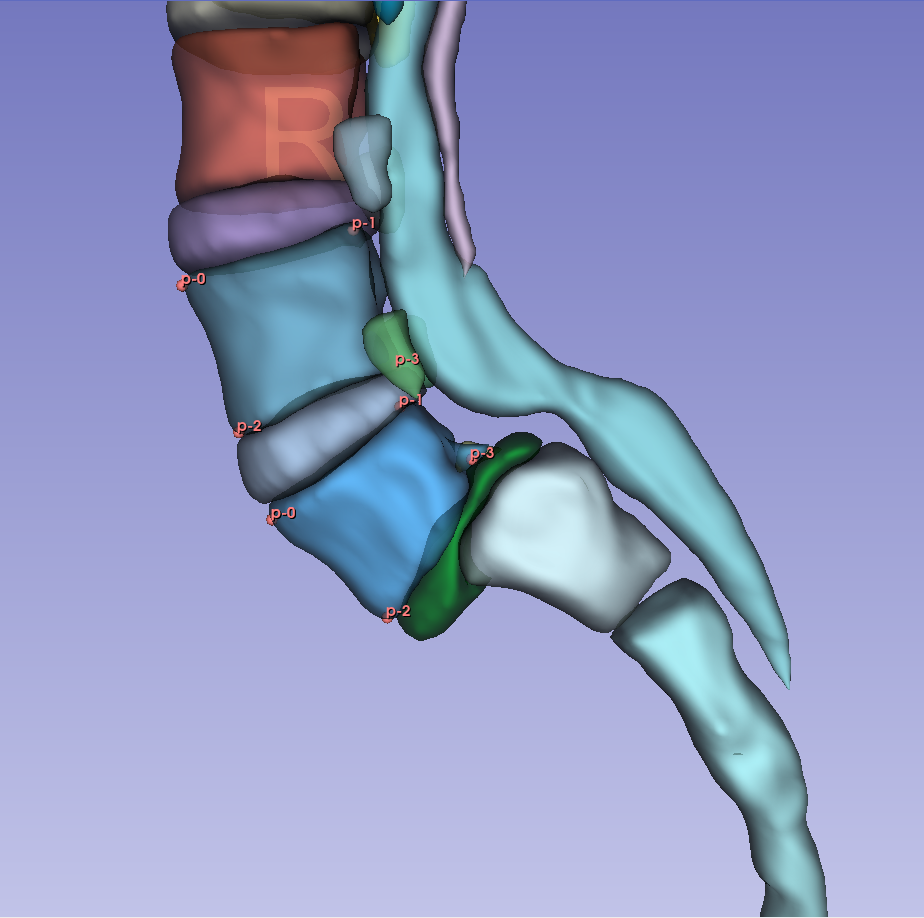
\includegraphics[width=1\textwidth]{obrazy/kregozmyk_kontur.png}
    \captionsetup{justification=centering, font=small}
    \caption{Wyznaczone narożne punkty kręgów L4 i L5}
    \label{fig:spondylolisthesis-contour}
\end{figure}

\subsection{Wyznaczenie znormalizowanego przesunięcia strzałkowego}
\label{subsec:przesuniecie}

Dla analizowanej pary kręgów, oznaczonych jako $V_g$ (kręg górny) oraz $V_d$ (kręg dolny), spośród wyznaczonych wcześniej punktów narożnych wybierane są trzy:

\begin{itemize}
    \item $P_A$ -- tylny narożnik górnej płytki granicznej kręgu dolnego $V_d$,
    \item $P_B$ -- przedni narożnik górnej płytki granicznej kręgu dolnego $V_d$,
    \item $P_P$ -- tylny narożnik dolnej płytki granicznej kręgu górnego $V_g$.
\end{itemize}

Rozróżnienie narożników przednich i tylnych wynika bezpośrednio z orientacji przekroju: pozioma oś obrazu pokrywa się z osią $\vec{z}$, zwróconą w stronę kanału kręgowego, a zatem ku tyłowi.
Punkt $P_A$ pełni rolę początku układu pomiarowego -- odpowiada tylnej krawędzi trzonu kręgu dolnego, czyli tej samej strukturze, którą radiolog wyznacza na bocznym zdjęciu rentgenowskim przy pomiarze metodą Meyerdinga.

Na podstawie wybranych punktów definiowane są dwa wektory.
Wektor $\vec{AB}$ opisuje górną płytkę graniczną kręgu dolnego i wyznacza kierunek, wzdłuż którego mierzone jest przemieszczenie:

\begin{equation} \label{eq:ab-vector}
    \vec{AB} = P_B - P_A
\end{equation}

Wektor $\vec{AP}$ łączy tylne narożniki obu trzonów i reprezentuje pełne przemieszczenie przestrzenne kręgu górnego względem dolnego:

\begin{equation} \label{eq:ap-vector}
    \vec{AP} = P_P - P_A
\end{equation}


\begin{figure}[H]
    \centering
    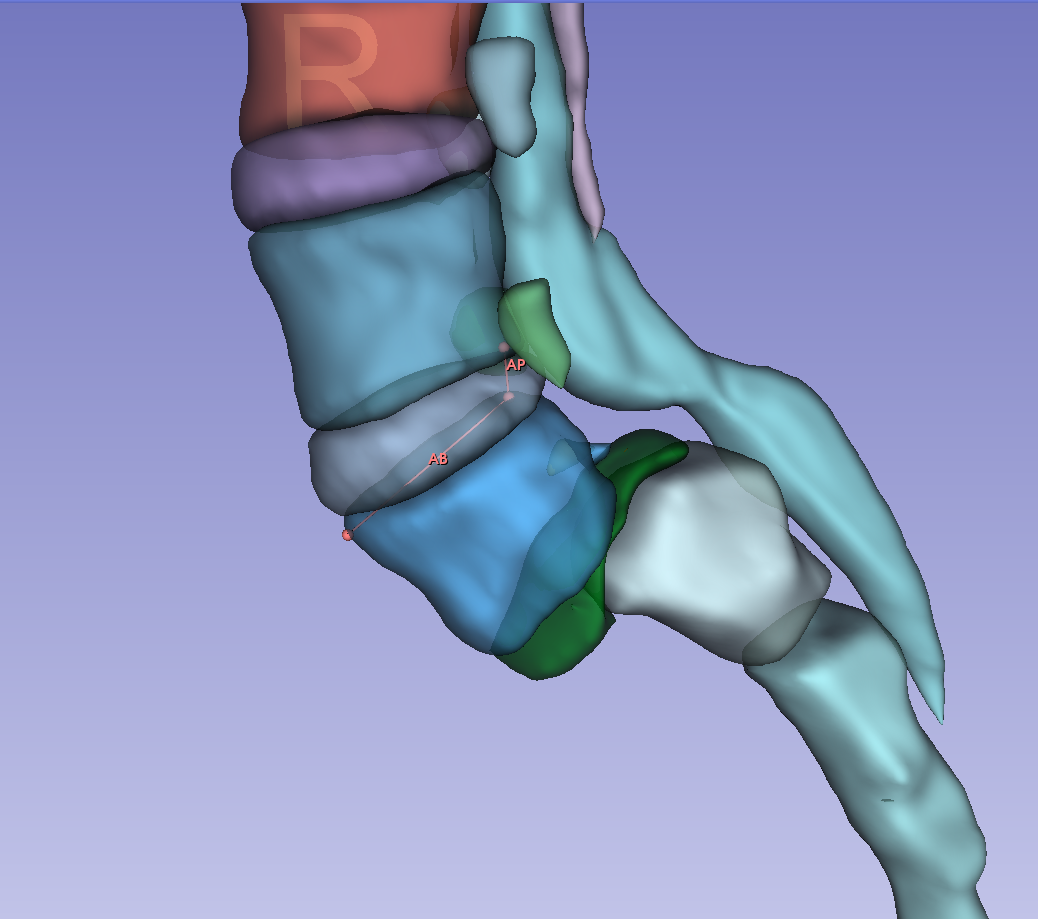
\includegraphics[width=1\textwidth]{obrazy/kregozmyk_wektory.png}
    \captionsetup{justification=centering, font=small}
    \caption{Wyznaczone wektory $\vec{AB}$ i $\vec{AP}$}
    \label{fig:spondylolisthesis-vectors}
\end{figure}

Wektor $\vec{AP}$ zawiera składowe we wszystkich trzech kierunkach, w tym składową pionową odpowiadającą wysokości krążka międzykręgowego oraz ewentualną składową boczną.
Wielkością diagnostyczną jest wyłącznie składowa równoległa do płytki granicznej, dlatego wyznaczany jest rzut prostopadły punktu $P_P$ na prostą zawierającą wektor $\vec{AB}$:

\begin{equation} \label{eq:projection}
    P_{rzut} = P_A + \frac{\vec{AP} \cdot \vec{AB}}{\vec{AB} \cdot \vec{AB}} \, \vec{AB}
\end{equation}

Wektor przemieszczenia $\vec{d}$ zdefiniowany jest jako różnica położenia rzutu i punktu odniesienia:

\begin{equation} \label{eq:displacement}
    \vec{d} = P_{rzut} - P_A
\end{equation}

\begin{figure}[H]
    \centering
    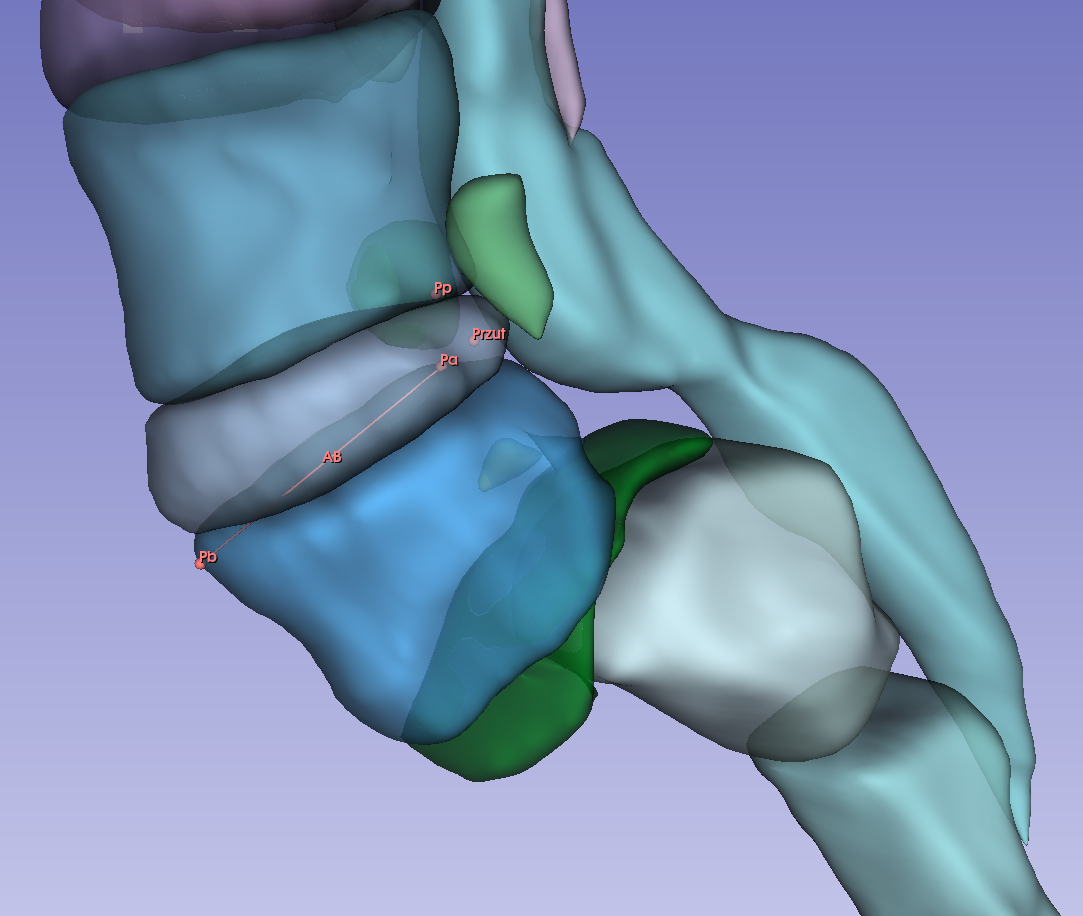
\includegraphics[width=1\textwidth]{obrazy/kregozmyk_point.png}
    \captionsetup{justification=centering, font=small}
    \caption{Przerzutowany punkt $P_{rzut}$ w odniesieniu do $P_A$, $P_B$ i $P_P$}
    \label{fig:spondylolisthesis-point}
\end{figure}

Operacja rzutowania realizuje jednocześnie dwa cele.
Po pierwsze, eliminuje składowe przemieszczenia nieistotne z punktu widzenia rozpoznania, sprowadzając pomiar do jednego wymiaru.
Po drugie, ponieważ wykonywana jest w fizycznej przestrzeni trójwymiarowej, jej wynik nie zależy od globalnej orientacji kręgosłupa w przestrzeni skanera ani od ułożenia pacjenta podczas badania.

Ostateczna wartość pomiaru wyrażana jest jako iloraz długości wektora przemieszczenia oraz szerokości górnej płytki granicznej kręgu dolnego:

\begin{equation} \label{eq:normalized-slip}
    s = \frac{\|\vec{d}\|}{\|\vec{AB}\|}
\end{equation}

Wielkość $s$ jest bezwymiarowa, przez co pozostaje niewrażliwa na rozdzielczość przestrzenną badania oraz na indywidualne różnice w wielkości kręgów u poszczególnych pacjentów.
Odpowiada ona bezpośrednio odsetkowi przemieszczenia stosowanemu w skali Meyerdinga (tabela~\ref{tab:meyerding}), przy czym w metodzie klasycznej mianownikiem jest szerokość górnej powierzchni kręgu leżącego poniżej, mierzona na dwuwymiarowym zdjęciu rentgenowskim, a w opisywanym algorytmie -- długość odcinka łączącego tylny i przedni narożnik tej samej płytki, wyznaczona w przestrzeni trójwymiarowej.

\subsection{Klasyfikacja kierunku przesunięcia}
\label{subsec:kierunek}

Wielkość $s$ zdefiniowana równaniem~\eqref{eq:normalized-slip} jest nieujemna, nie rozróżnia zatem przemieszczenia przedniego od tylnego.
Kierunek ześlizgu wyznaczany jest na podstawie znaku iloczynu skalarnego wektora przemieszczenia $\vec{d}$ oraz wektora płytki granicznej $\vec{AB}$:

\begin{equation} \label{eq:direction-sign}
    c = \vec{d} \cdot \vec{AB}
\end{equation}

Wektor $\vec{AB}$ zwrócony jest od tylnego narożnika trzonu ku przedniemu, czyli w kierunku brzusznym.
Dodatnia wartość $c$ oznacza zatem, że tylna krawędź kręgu górnego przemieszczona jest ku przodowi względem tylnej krawędzi kręgu dolnego, co odpowiada kręgozmykowi.
Ujemna wartość $c$ wskazuje na przemieszczenie ku tyłowi, czyli na tyłozmyk:

\begin{equation} \label{eq:classification}
    \text{rozpoznanie} =
    \begin{cases}
        \text{kręgozmyk} & \text{jeżeli } c > 0 \\
        \text{tyłozmyk}  & \text{w przeciwnym razie}
    \end{cases}
\end{equation}

Poprawność takiej klasyfikacji opiera się na zwrocie osi $\vec{z}$, wyznaczonym w sposób opisany w podrozdziale~\ref{subsec:wspolne-etapy}.
Ponieważ kanał kręgowy znajduje się zawsze grzbietowo względem trzonu, wektor prowadzony od centroidu trzonu do najbliższego punktu kanału jednoznacznie wskazuje kierunek tylny, niezależnie od orientacji pacjenta w przestrzeni skanera oraz od konwencji zapisu układu współrzędnych w pliku wejściowym.

\subsection{Analiza wszystkich par kręgów}
\label{subsec:pary-kregow}

Pomiar wykonywany jest dla wszystkich par kręgów sąsiadujących ze sobą w analizowanym odcinku, to jest dla par Th11/Th12, Th12/L1, L1/L2, L2/L3, L3/L4, L4/L5 oraz L5/S1.
Ograniczenie do par sąsiednich wynika z definicji klinicznej: kręgozmyk jest przemieszczeniem względem kręgu bezpośrednio niżej położonego i opisywany jest zawsze na konkretnym poziomie ruchowym, w przeciwieństwie do skrzywienia skoliotycznego, które obejmuje wiele poziomów jednocześnie.

Wynikiem działania algorytmu jest zbiór trójek $(poziom, kierunek, s)$ -- po jednej dla każdej pary obecnej w segmentacji.
Wartości te nie są uśredniane ani agregowane do pojedynczej liczby, ponieważ rozpoznanie kliniczne formułowane jest osobno dla każdego poziomu, a jeden pacjent może wykazywać kręgozmyk na jednym poziomie i tyłozmyk na innym.
Zestawienie takie odpowiada strukturą opisowi radiologicznemu badania.

Przypisanie stopnia w skali Meyerdinga (tabela~\ref{tab:meyerding}) wynika bezpośrednio z wartości $s$: stopień I odpowiada przedziałowi $s \in [0{,}00;\, 0{,}25)$, stopień II -- $[0{,}25;\, 0{,}50)$, stopień III -- $[0{,}50;\, 0{,}75)$, a stopień IV -- $[0{,}75;\, 1{,}00]$.
Kwalifikacja przypadku jako patologicznego wymaga natomiast przyjęcia wartości progowej oddzielającej fizjologiczną zmienność położenia trzonów od rzeczywistego ześlizgu, ponieważ nawet w kręgosłupie prawidłowym wyznaczona wartość $s$ jest niezerowa.
Dobór tej wartości na podstawie zbioru badań referencyjnych omówiono w rozdziale poświęconym analizie wyników.

Wyniki pomiaru wraz z punktami pośrednimi -- narożnikami trzonów, wektorami $\vec{AB}$ i $\vec{AP}$ oraz punktem rzutu $P_{rzut}$ -- zapisywane są w formacie JSON zgodnym ze schematem \textit{Markups} oprogramowania 3D~Slicer.
Umożliwia to nałożenie wyników pośrednich na oryginalne badanie i wizualną weryfikację poprawności każdego etapu przetwarzania.

\subsection{Złożoność obliczeniowa}
\label{subsec:zlozonosc}

Niech $V$ oznacza liczbę wokseli wolumenu wejściowego, $N$ -- liczbę punktów linii środkowej kanału kręgowego, a $K$ -- liczbę kręgów obecnych w segmentacji ($K \leq 8$).

Etap przygotowania kanału kręgowego zdominowany jest przez operacje wolumetryczne: zamknięcie morfologiczne oraz szkieletyzację metodą Lee, których koszt jest liniowy względem liczby wokseli, czyli $O(V)$.
Interpolacja funkcjami sklejanymi oraz reparametryzacja krzywej mają złożoność $O(N)$, przy czym $N$ jest o kilka rzędów wielkości mniejsze od $V$.

Dla każdego kręgu wykonywane jest wyszukiwanie najbliższego punktu kanału metodą przeglądu zupełnego, o koszcie $O(N)$, oraz przepróbkowanie przekroju o stałym rozmiarze $500 \times 500$ pikseli.
Operacje wizji komputerowej -- otwarcie morfologiczne, detekcja krawędzi, wyznaczenie otoczki wypukłej i aproksymacja wielokątowa -- działają na obrazie o stałym rozmiarze, ich koszt jest zatem stały względem rozmiaru danych wejściowych.
Łączny koszt etapu analizy kręgów wynosi $O(K \cdot N)$.

Sam pomiar przesunięcia sprowadza się do kilku operacji wektorowych na trzech punktach, wykonywanych $K-1$ razy, a więc jego udział w całkowitym czasie przetwarzania jest pomijalny.
Warto zaznaczyć, że w tym punkcie algorytm jest istotnie tańszy obliczeniowo od algorytmu detekcji skoliozy: tam analizowane są wszystkie pary kręgów spełniające warunek $j \geq i+2$, co daje liczbę kombinacji rosnącą kwadratowo z liczbą kręgów, natomiast tutaj rozpatrywanych jest jedynie $K-1$ par sąsiednich.
Ostatecznie złożoność całego algorytmu wynosi $O(V + K \cdot N)$ i pozostaje zdominowana przez wolumetryczne operacje wstępnego przetwarzania.
